\chapter{Completed Work}


%%%%%%%%%%%%%%   Overview over article should not include too much equations
%%  bottom line - take home message - the derivations should ref the article

%%  
%%  remove the techinalities - 
%%     using the procedure we have calculated for.. blah blah
%%       see figure. (leave plots only if neccessary to buttom line).
%%
%%  geometry plots - maybe try with normal scale.
%%                   if that doesn't work, leave the figure out.


%%%%%%%%%%%%%%%%%%%%%%%%%
\section{The $d=1$ random site model with nearest neighbor hopping}

In $d=1$, a network with randomly distributed sites is equivalent to
an ordered lattice with random transition rates. To make this mapping
we have to know the spacing distribution for this system. We find the
spacing distribution in \autoref{sec:spacing}. A $1d$ lattice with
a known transition rates distribution is exactly solvable \cite{alexander_excitation_1981}.
Basically, it is analogous to adding connectors in series, and 
the diffusion coefficient is the inverse of the combined resistivity
%
\begin{align}
D \ =\ \left(\frac{1}{N} \sum_n \frac{1}{w_{n,n-1}}\right)^{-1}
\end{align}
%
The rates are 
%
\begin{align}
w_{n,n-1} \ =\ w_0 \eexp{-r_{n,n-1}/\xi}
\end{align}
Using the spacing distribution from \autoref{eq:spacing_dist}, we can change distribution variables
from $r$ to $w$. Defining $s \equiv \xi/r_0$ and converting the sum to an integral, we obtain
%
\begin{align}
D \ =\ \left(\frac{1}{N} \int_0^{w_0} \frac{s w^{s-1}dw}{w_0^s}\right)^{-1} \
\ =\ [s>1]\quad \frac{s-1}{s}w_0
\end{align}
% TODO : something is wrong with the N in this expression
This result is valid only for $s>1$. For $s<1$, $D=0$ and we have
subdiffusion, for which the survival probability and spreading 
are also exactly solvable \cite{alexander_excitation_1981}, leading to:
%
\begin{align}
S(t)           \ &\sim \ t^{2s/(1+s)} \\
\mathcal{P}(t) \ &\sim \ t^{-s/(1+s)}
\end{align}
%
%%%%%%%%%%%%%%%%%%%
\section{The ERH - Effective Range Hopping - procedure}

The diffusion coefficient is defined by the dependence
of the variance in time:
%
\begin{align}
\textrm{Var}(n) \quad =\quad 2d\ D\ t
\end{align}
%
Within the transient diffusion stage,
assuming we start at a specific node $n$, the variance after time
$t$ will be
%
\begin{align}
\textrm{Var}(n) = \sum_m w_{nm} t (x_m-x_n)^2
\end{align}
Therefore, the diffusion coefficient for evolution 
starting at node $n$ is
%
\begin{align}
D_n \quad=\quad \frac{1}{2d}\sum_m (x_m-x_n)^2 w_{nm}
\end{align}
%
Averaging over the starting node, and converting the sum to an integral,
we have
%
\begin{align}\label{eq:linear_D}
D_{\tbox{linear}}  \ \ = \ \ \frac{1}{2d}\iint w(r,\epsilon) \ r^2  \ \rho(r,\epsilon) \ d\epsilon dr 
\end{align}
%

This expression describes the spreading in absence of disorder correctly
for arbitrary long time. However, in a sparse disordered system such as ours,
the possibility of transport is a bit less trivial. Therefore, we suggest
a method to approximate the diffusion, which takes percolation into account.


The basic idea behind \emph{ERH} is that in the linear
expression, nearby sites 
with $r\ll 1$ (and therefore $w \gg 1$ ) are over represented in
the diffusion coefficient calculation. While the transition to
these sites is indeed high, the distance covered is not enough
to form a percolating cluster. Therefore, we use a threshold based
on percolation theory and flat-down the rates higher then this threshold.

The rate threshold $w_c$ is determined using the following expression
%
\begin{align}\label{eq:threshold}
\iint_{w(r,\epsilon)>w_c} \rho(r,\epsilon)drd\epsilon \ \ = \ \ n_c
\end{align}
%
Where $n_c$ is the number of connected sites necessary to form a percolation
cluster.


Next, we suppress the rates higher than $w_c$ to have the value $w_c$,
and use the linear expression \ref{eq:linear_D}, to obtain:
%
\begin{align}\label{eq:ERH_D}
D_{\tbox{ERH}} = \frac{1}{2d}\iint \min\{w(r,\epsilon),w_c\} \ r^2  \ \rho(r,\epsilon) \ d\epsilon dr
\end{align}
%


Using the ERH procedure we have calculated the diffusion for several models.


For the $d=2$ ordered lattice with nearest neighbor random hopping:
%
\begin{align}
D_{\tbox{ERH}} =  \left[\frac{1}{2}w_c + \frac{1}{2}\int_0^{w_c} w\tilde{f}(w) dw\right]r_0^2
\end{align}
%
In absence of the disorder (i.e.\ all the rates are equal),
the known result $D = w_0r_0^2$ is restored.


For the degenerate hopping model, 

\begin{align}
D_{\tbox{ERH}} &=  \mathrm{EXP}_{d{+}2}\left(\frac{1}{s_c}\right)  \  \eexp{-1/s_c}  \ D_{\tbox{linear}}
\end{align}
%


For the Mott Hopping model,
%
\begin{align}
D_{\tbox{ERH}} &=\mathrm{EXP}_{d{+}3}\left(\epsilon_c\right)  \  \eexp{-\epsilon_c}  \ D_{\tbox{linear}}
\end{align}
%


For the flat-profile banded $1d$ model,
\begin{align}
D_{\text{ERH}} \ \ = \ \ 
\ \frac{1}{\sigma}\left[ 
\left(1+\frac{n_c}{2b}\sigma\right)\eexp{-\frac{n_c}{2b}\sigma} - \eexp{-2\sigma}
\right] \ \tilde{b} w_0
\end{align}

%%%%%%%%%%%%%%%%%%%%%%%%%%%%%%%%%%%%%%%%%%%%%%%%%%%%
%%%%%%%%%%%%%%%%%%%%%%%%%%%%%%%%%%%%%%%%%%%%%%%%%%%%
\chapter{Preliminary analysis}




%%%%%%%%   I need to add dts.tex here.
%%%%%%%%   I could also add D(g_s) and say that it failed

%%%%%%%%%%%%%%%%%%%%%%%%%%%%%
\section{The quasi one dimensional Hamiltonian}


In this model , described in \autoref{sec:quasi_bg}, initial analysis of
the numerical results reveals that the sparsity affects the diffusion coefficient.
We see that as the system becomes more sparse, the diffusion coefficient is suppressed. 
As might be expected, the lower bandwidth ensembles are more
susceptible, as the system is more vulnerable to disconnections.



\begin{figure}
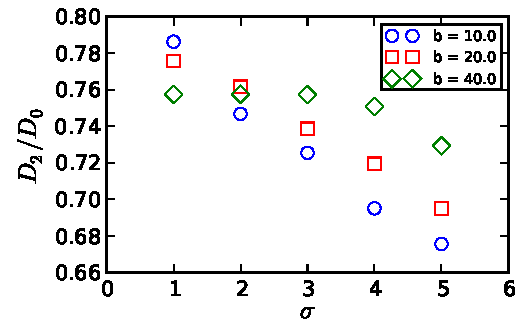
\includegraphics{dts_D2}
\caption{The transient diffusion coefficient for quantum spreading in
a banded sparse network. The ratio $D/D_0$ between the numerical diffusion 
coefficient and the expected value decreases as $\sigma$ increases. The effect
is stronger for low bandwidth.}
\end{figure}
